% The lattice of fields between ℚ and ℚ(√2, √3) alongside the lattice
% of subgroups of its Klein-four Galois group, illustrating the
% fundamental theorem of Galois theory.
% Source: book/tex/alg-NT/galois.tex (§ Fundamental theorem of Galois
% theory) — two tikzcds.
\documentclass[border=2mm]{standalone}
\usepackage{tikz}
\usepackage{amssymb}
\begin{document}
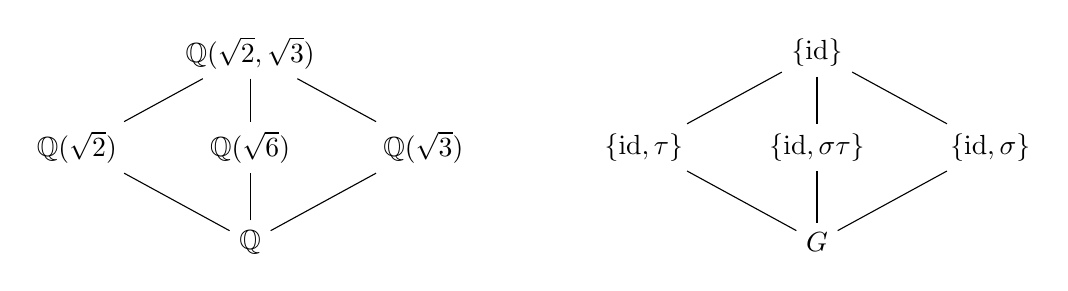
\begin{tikzpicture}
  \begin{scope}
    \node (top) at (0,2.4) {$\mathbb{Q}(\sqrt2,\sqrt3)$};
    \node (l) at (-2.2,1.2) {$\mathbb{Q}(\sqrt2)$};
    \node (m) at (0,1.2) {$\mathbb{Q}(\sqrt6)$};
    \node (r) at (2.2,1.2) {$\mathbb{Q}(\sqrt3)$};
    \node (bot) at (0,0) {$\mathbb{Q}$};
    \draw (top) -- (l); \draw (top) -- (m); \draw (top) -- (r);
    \draw (bot) -- (l); \draw (bot) -- (m); \draw (bot) -- (r);
  \end{scope}
  \begin{scope}[shift={(7.2,0)}]
    \node (top) at (0,2.4) {$\{\mathrm{id}\}$};
    \node (l) at (-2.2,1.2) {$\{\mathrm{id},\tau\}$};
    \node (m) at (0,1.2) {$\{\mathrm{id},\sigma\tau\}$};
    \node (r) at (2.2,1.2) {$\{\mathrm{id},\sigma\}$};
    \node (bot) at (0,0) {$G$};
    \draw (top) -- (l); \draw (top) -- (m); \draw (top) -- (r);
    \draw (bot) -- (l); \draw (bot) -- (m); \draw (bot) -- (r);
  \end{scope}
\end{tikzpicture}
\end{document}
